\newpage

\begin{table}[h]
\caption{Standardized selection gradients acting on \textit{Iteomyia} in complex vs. simple food webs.}
\label{Table:Gradients}
\centering
\begin{tabular}{lccc}
\\ 
\hline
\textbf{Selection gradient} & \textbf{Complex} & \textbf{Simple} & \textbf{Contrast}  \\ 
\hline
$\beta_{\text{Diam}}$ & 
\textbf{
0.36 [
0.22,
0.51] }& 
\textbf{
0.21 [
0.11,
0.31] }& 
\textbf{
-0.15 [
-0.31,
0.01] }\\

$\beta_{\text{Clutch}}$ & 
0.04 [
-0.07,
0.17] & 
\textbf{
-0.16 [
-0.26,
-0.08] }& 
\textbf{
-0.21 [
-0.38,
-0.07] }\\

$\beta_{\text{Pref}}$ &
\textbf{
-0.2 [
-0.37,
-0.04] }& 
\textbf{
-0.19 [
-0.3,
-0.1] }& 

0.01 [
-0.2,
0.19] \\

$\gamma_{\text{Diam,Diam}}$ &
0.13 [
-0.02,
0.29] & 

0.1 [
-0.02,
0.25] & 

-0.03 [
-0.22,
0.16] \\

$\gamma_{\text{Clutch,Clutch}}$ & 
-0.04 [
-0.26,
0.16] & 

-0.12 [
-0.26,
0.02] & 

-0.08 [
-0.32,
0.14] \\

$\gamma_{\text{Pref,Pref}}$ & 
\textbf{
0.33 [
0.1,
0.59] }& 

0.03 [
-0.13,
0.18] & 
\textbf{
-0.3 [
-0.62,
-0.06] }\\

$\gamma_{\text{Diam,Clutch}}$ & 
-0.04 [
-0.16,
0.08] & 

-0.07 [
-0.14,
0.02] & 

-0.03 [
-0.16,
0.11] \\

$\gamma_{\text{Diam,Pref}}$ & 
\textbf{
-0.11 [
-0.24,
0.03] }& 

-0.02 [
-0.1,
0.05] & 

0.1 [
-0.07,
0.27] \\

$\gamma_{\text{Clutch,Pref}}$ & 
0.01 [
-0.13,
0.15] & 

0 [
-0.06,
0.07] & 

-0.01 [
-0.18,
0.15] \\ 
\hline
\end{tabular}
\bigskip{}
\\
{\footnotesize Note: Values in brackets represent 95\% confidence intervals. $\beta_{\text{Diam}}$ has been adjusted for bias.}
\end{table}

\begin{table}[h]
\caption{Relationship between absolute fitness (larva survival) and phenotypic traits of \textit{Iteomyia} in complex vs. simple food webs.}
\label{Table:Coefs}
\centering
\begin{tabular}{lccc}
\\ 
\hline
\textbf{Coefficient} & \textbf{Complex} & \textbf{Simple} & \textbf{Contrast}  \\ 
\hline
$\alpha_{\text{Diam}}$ & 
\textbf{
1.19 [
0.73,
1.71] }& 
\textbf{
1.11 [
0.6,
1.67] }& 

-0.08 [
-0.66,
0.55] \\

$\alpha_{\text{Clutch}}$ & 
0.14 [
-0.25,
0.57] & 
\textbf{
-0.87 [
-1.4,
-0.41] }& 
\textbf{
-1.01 [
-1.81,
-0.41] }\\

$\alpha_{\text{Pref}}$ &
\textbf{
-0.65 [
-1.25,
-0.12] }& 
\textbf{
-1.01 [
-1.6,
-0.53] }& 

-0.36 [
-1.25,
0.3] \\

$\alpha_{\text{Diam,Diam}}$ &
0.21 [
-0.03,
0.48] & 

0.26 [
-0.06,
0.67] & 

0.05 [
-0.33,
0.45] \\

$\alpha_{\text{Clutch,Clutch}}$ & 
-0.06 [
-0.44,
0.27] & 

-0.32 [
-0.69,
0.05] & 

-0.25 [
-0.68,
0.2] \\

$\alpha_{\text{Pref,Pref}}$ & 
\textbf{
0.56 [
0.17,
0.99] }& 

0.08 [
-0.35,
0.47] & 
\textbf{
-0.48 [
-1.07,
0.04] }\\

$\alpha_{\text{Diam,Clutch}}$ & 
-0.13 [
-0.53,
0.25] & 

-0.36 [
-0.76,
0.09] & 

-0.23 [
-0.81,
0.37] \\

$\alpha_{\text{Diam,Pref}}$ & 
\textbf{
-0.38 [
-0.8,
0.08] }& 

-0.1 [
-0.52,
0.27] & 

0.28 [
-0.31,
0.92] \\

$\alpha_{\text{Clutch,Pref}}$ & 
0.04 [
-0.42,
0.5] & 

0.01 [
-0.33,
0.37] & 

-0.03 [
-0.7,
0.56] \\ 
\hline
\end{tabular}
\bigskip{}
\\
{\footnotesize Note: Values in brackets represent 95\% confidence intervals. $\alpha_{\text{Diam}}$ has been adjusted for bias.}
\end{table}

\section*{Figure legends}

\begin{figure}
\centering
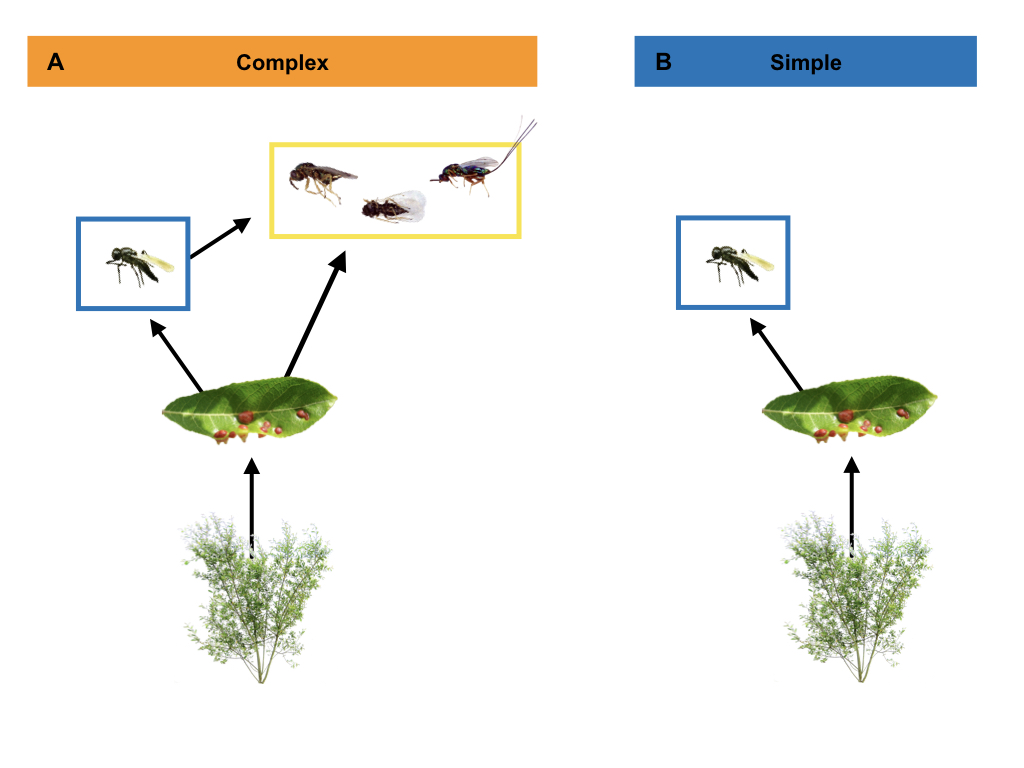
\includegraphics{analyses/complex_simple_foodwebs.jpeg}
\caption{\label{fig:Conceptual}Illustrations of complex (A) and simple
(B) food webs associated with the insect herbivore, \emph{Iteomyia
salicisverruca}. Black arrows denote the flow of energy in this network
of trophic interactions.}
\end{figure}
